\begin{figure*}[t!]
  \centering
% \hspace{-0.2in}
  \begin{subfigure}{0.24\textwidth}
    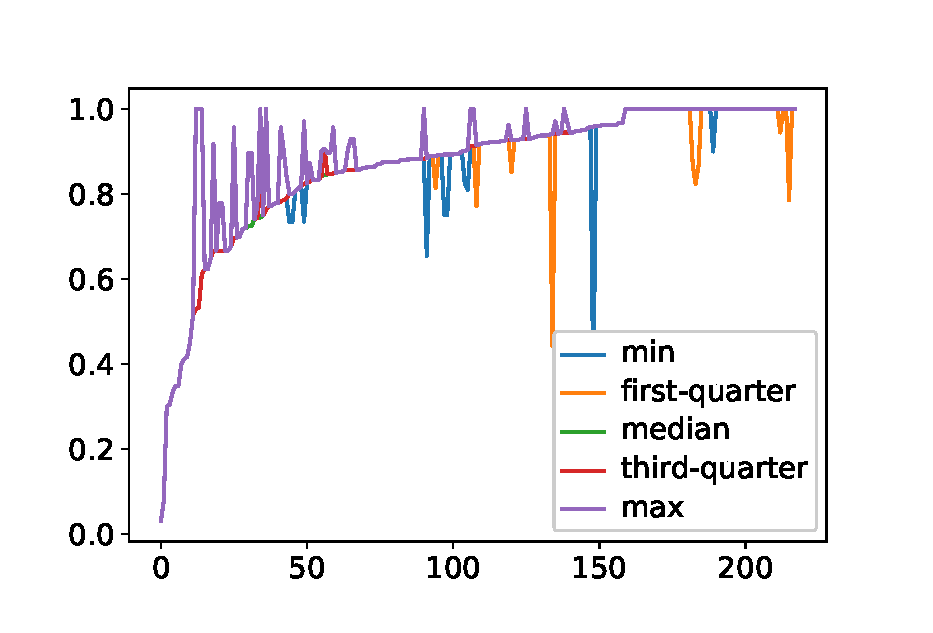
\includegraphics[width=4.8cm]{figure/trend-bug.eps}
	 \caption{Trend \%bug}
	 \label{fig:trend-b}
  \end{subfigure}
%  \hspace{-0.1in}
  \begin{subfigure}{0.24\textwidth}
    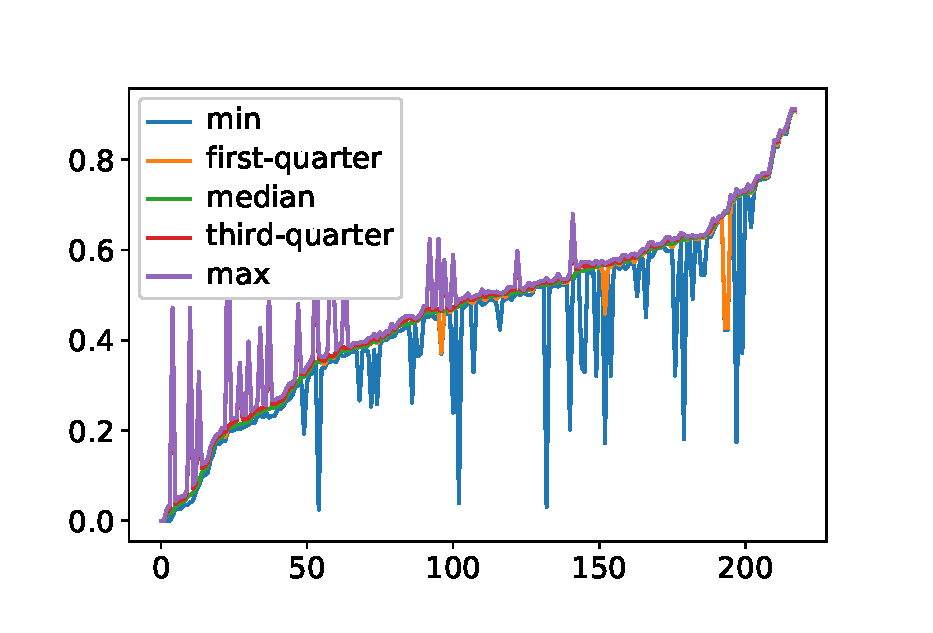
\includegraphics[width=4.8cm]{figure/trend-cost.eps}
	\caption{Trend \%reducedCost}
   \label{fig:trend-c}
  \end{subfigure}
  \begin{subfigure}{0.24\textwidth}
    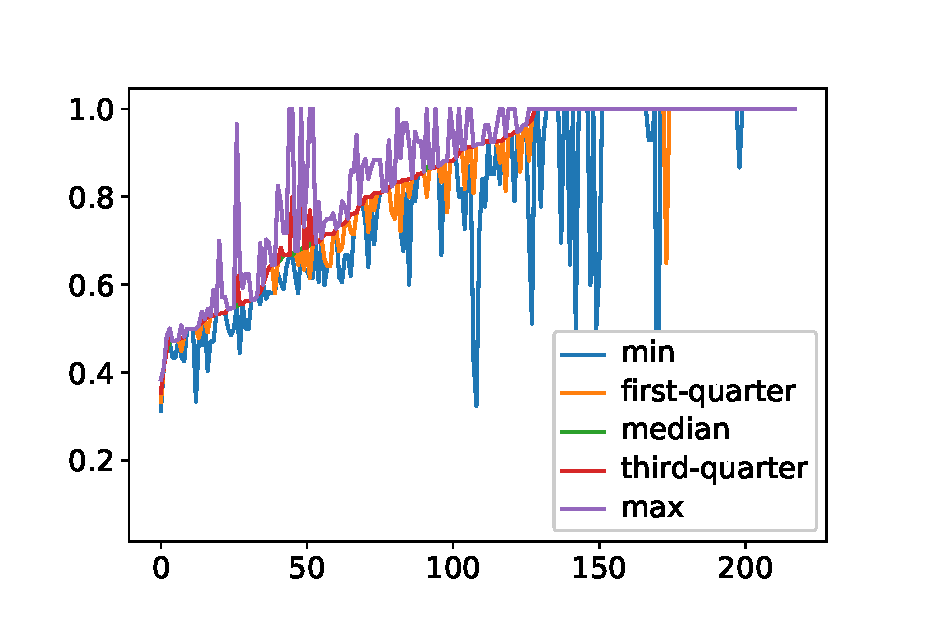
\includegraphics[width=4.8cm]{figure/arrival-bug.eps}
	\caption{Peak \%bug}
    \label{fig:peak-b}
  \end{subfigure}
  \begin{subfigure}{0.24\textwidth}
    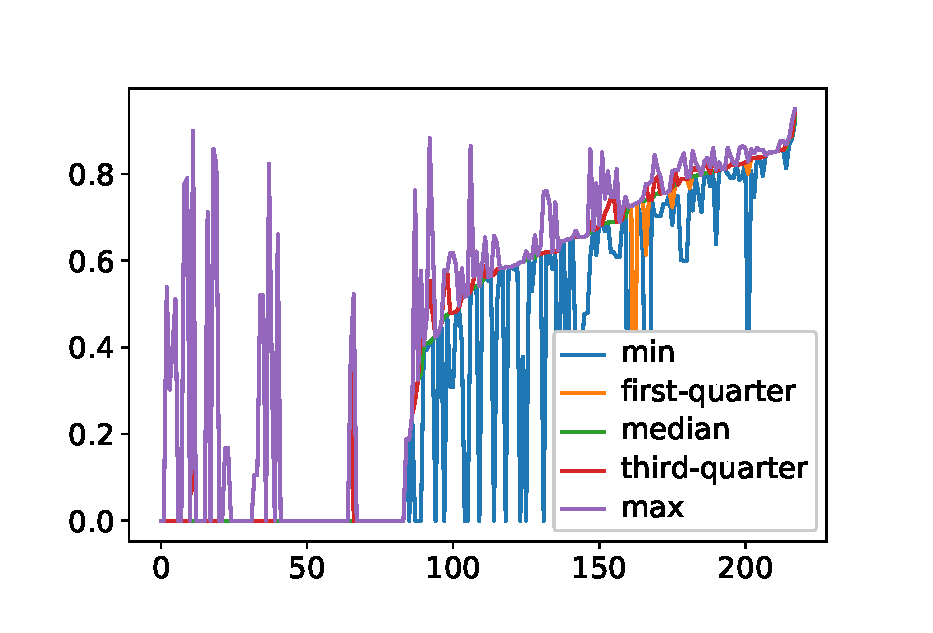
\includegraphics[width=4.8cm]{figure/arrival-cost.eps}
	\caption{Peak \%reducedCost}
    \label{fig:peak-c}
  \end{subfigure}
  \begin{subfigure}{0.24\textwidth}
    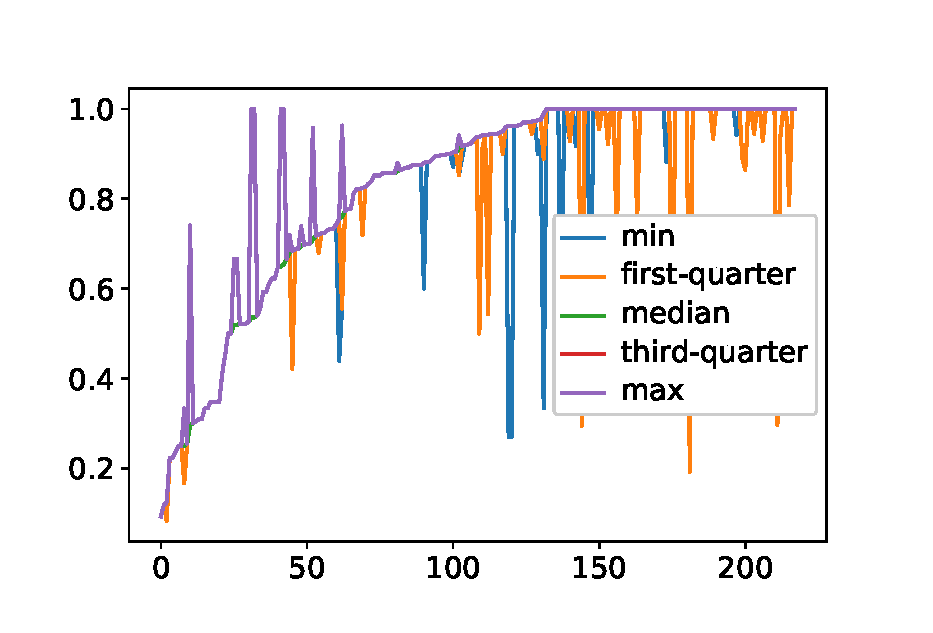
\includegraphics[width=4.8cm]{figure/knee-bug.eps}
	 \caption{Knee \%bug}
	 \label{fig:knee-b}
  \end{subfigure}
%  \hspace{-0.1in}
  \begin{subfigure}{0.24\textwidth}
    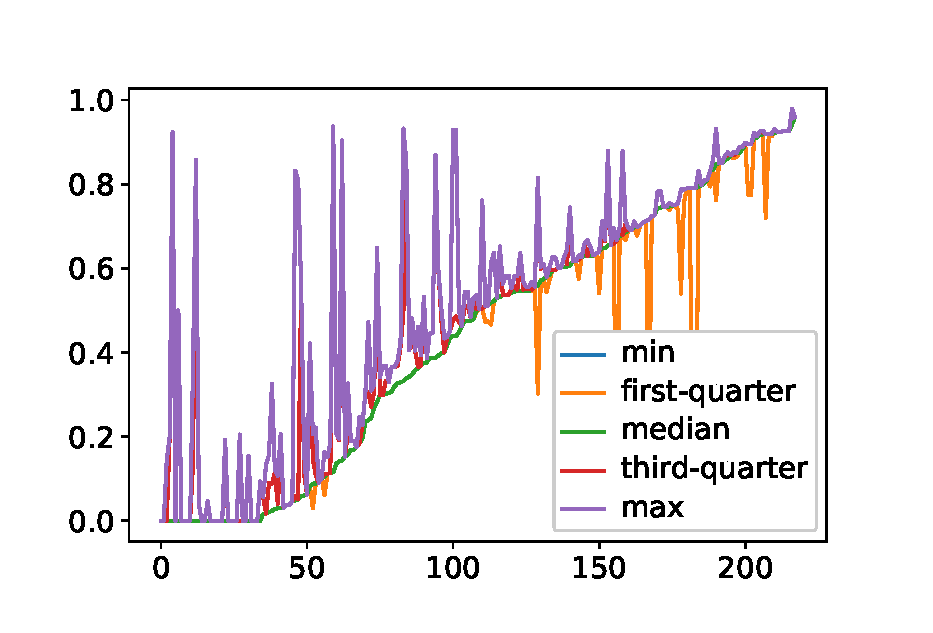
\includegraphics[width=4.8cm]{figure/knee-cost.eps}
	\caption{Knee \%reducedCost}
   \label{fig:knee-c}
  \end{subfigure}
  \begin{subfigure}{0.24\textwidth}
    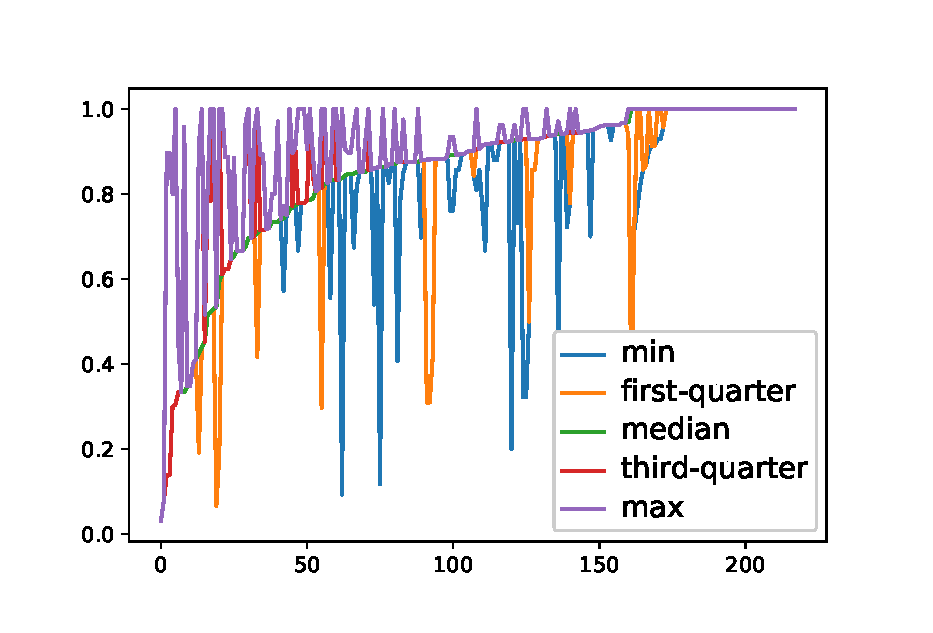
\includegraphics[width=4.8cm]{figure/M0-bug.eps}
	\caption{M0 \%bug}
    \label{fig:m0-b}
  \end{subfigure}
  \begin{subfigure}{0.24\textwidth}
    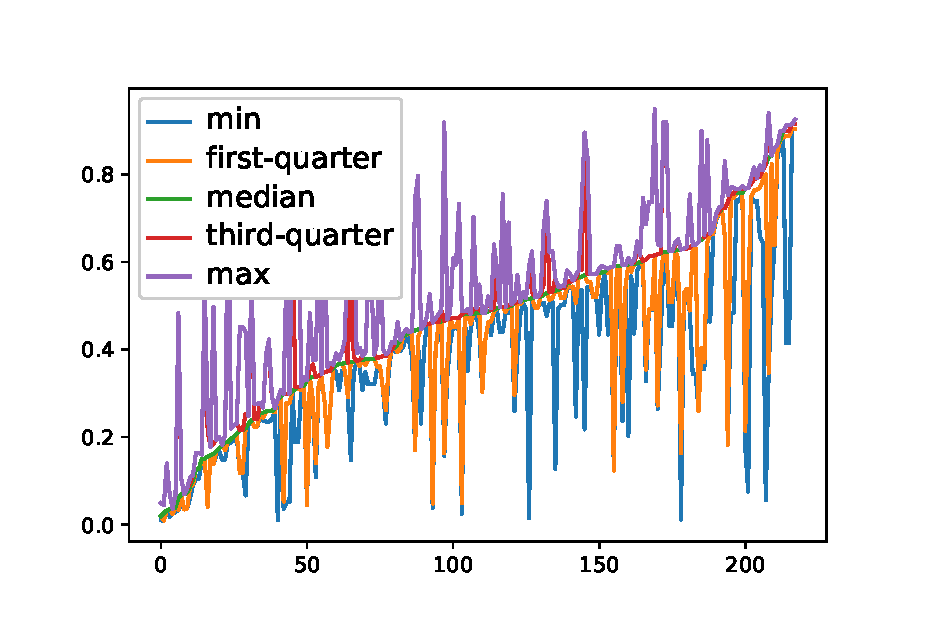
\includegraphics[width=4.8cm]{figure/M0-cost.eps}
	\caption{M0 \%reducedCost}
    \label{fig:m0-c}
  \end{subfigure}
  \caption{Stability of performance in terms of 1000 cross validations }
  \label{fig:random}
\vspace{-0.1in}
\end{figure*}


